\documentclass[11pt]{article}

\usepackage{acl2013}
\usepackage{times}
\usepackage{latexsym}
\usepackage{amsmath}
\usepackage{multirow}
\usepackage{array}
\usepackage{url}
\usepackage{graphicx}
\usepackage{subfig}
\usepackage{marvosym}
\usepackage{todonotes}

\setlength\titlebox{6.5cm}

\newcommand{\mnote}[1]{\marginpar{%
  \vskip-\baselineskip
  \raggedright\footnotesize
  \itshape\hrule\smallskip\footnotesize{#1}\par\smallskip\hrule}}

%% \newcommand{\aff}{\ensuremath{{}^\text{\Radioactivity}}}
%% \newcommand{\afff}{\ensuremath{{}^\text{\Bat}}}
\newcommand{\hltcoe}{\ensuremath{{}^\text{1}}}
\newcommand{\clsp}{\ensuremath{{}^\text{2}}}
\newcommand{\upenn}{\ensuremath{{}^\text{2}}}
\newcommand{\grammarrule}[3]{$#1 \to \langle \text{#2} , \text{#3} \rangle$ }

\title{Joshua 5.0: Every day, and in every way, getting better and better}

\author{Matt Post\hltcoe \and Juri Ganitkevitch\clsp \and Yuan Cao\clsp \and Jonathan Weese\clsp 
  \and Luke Orland\hltcoe \\
  \clsp Center for Language and Speech Processing \\
  \hltcoe Human Language Technology Center of Excellence \\
  Johns Hopkins University \\
  Baltimore, MD 21218
  \AND  Chris Callison-Burch \\
  Computer and Information Science \\
  University of Pennsylvania \\
  Philadelphia, PA 99999
}

\date{}

\begin{document}
\maketitle

\begin{abstract}

\end{abstract}

\section{Introduction}
\label{sec-intro}

What's new:

\begin{itemize}
  \item \emph{Sparse features and KBMIRA integration}.
  \item \emph{Pipeline improvements}.
  \item \emph{Thrax rewrite}. Find some way to show how much faster it is.
  \item \emph{Significantly faster}. Compare a graph over threads from last year to this year.
  \item \emph{Amortization}. Show how much faster that is.
  \item \emph{Server mode}. Show how that works.
  \item \emph{Synchronous parsing}. 
  \item \emph{Speed comparisons, contention elimination, etc}. Vary pruning settings and show model
    scores 
\end{itemize}

Joshua is an open-source toolkit\footnote{\url{joshua-decoder.org}}
for parsing-based statistical machine translation of human
languages. The original version of Joshua \cite{Joshua-WMT} was a port
(from Python to Java) of the Hiero machine translation system
\cite{Chiang2007}. It was later extended to support grammars with rich
syntactic labels \cite{li2010joshua}. Subsequent efforts produced
Thrax, the extensible Hadoop-based extraction tool for
synchronous context-free grammars \cite{Joshua-3.0}, which was later
extended to support pivoting-based paraphrase extraction
\cite{Joshua-4.0}.

Improvements in Joshua over the past year have been focused on speed
and usability.

%%%%%%%%%%%%%%%%%%%%%%%%%%%%%%%%%%%%%%%%%%%%%%%%%%%%%%%%%%%%%%%%%
\section{What's New in Joshua 5.0}

\subsection{Sparse features}

Until a few years ago, machine translation systems were for the most
part limited in the number of features they could employ, since the
line-based tuning method, MERT, was not able to efficiently search
over more than a few tens of feature weights. The introduction
large-scale discriminative tuning procedures has made it possible to
tune thousands of parameters simultaneously. Features of counts this
high are often sparse binary features, and so it becomes important to
be able to represent them internally in an efficient manner. 

Adding new sparse features is as easy as implementing the interface
depicted in Figure~\ref{figure:feature-api}. At each n-ary rule
application, all features are asked to score the rule. For performance
reasons, during construction of the chart, each feature only needs to
contribute a scalar value of the inner product of the weight vector
and the features incurred on that hyperedge. Afterwards, during k-best
extraction, a feature can return a more informative sparse feature
vector denoting the individual feature names and values incurred at
each edge.

For tuning large sets of features, Joshua supports both PRO
(introduced with Joshua 4.0) and batch MIRA.

\subsection{Performance improvements}

We introduced many performance improvements, replacing code designed
to get the job done under research timeline constraints with more
efficient alternatives. These improvements have led to speed increases
of up to 500\%, especially in multithreaded situations.
Figure~\ref{fig:cmp} plots end-to-end
runtime\footnote{i.e., including model loading time and grammar
  sorting.} Joshua 4.0 versus Joshua 5.0, as a function of the number
of threads.

\begin{figure}[!t]
  \begin{center}
    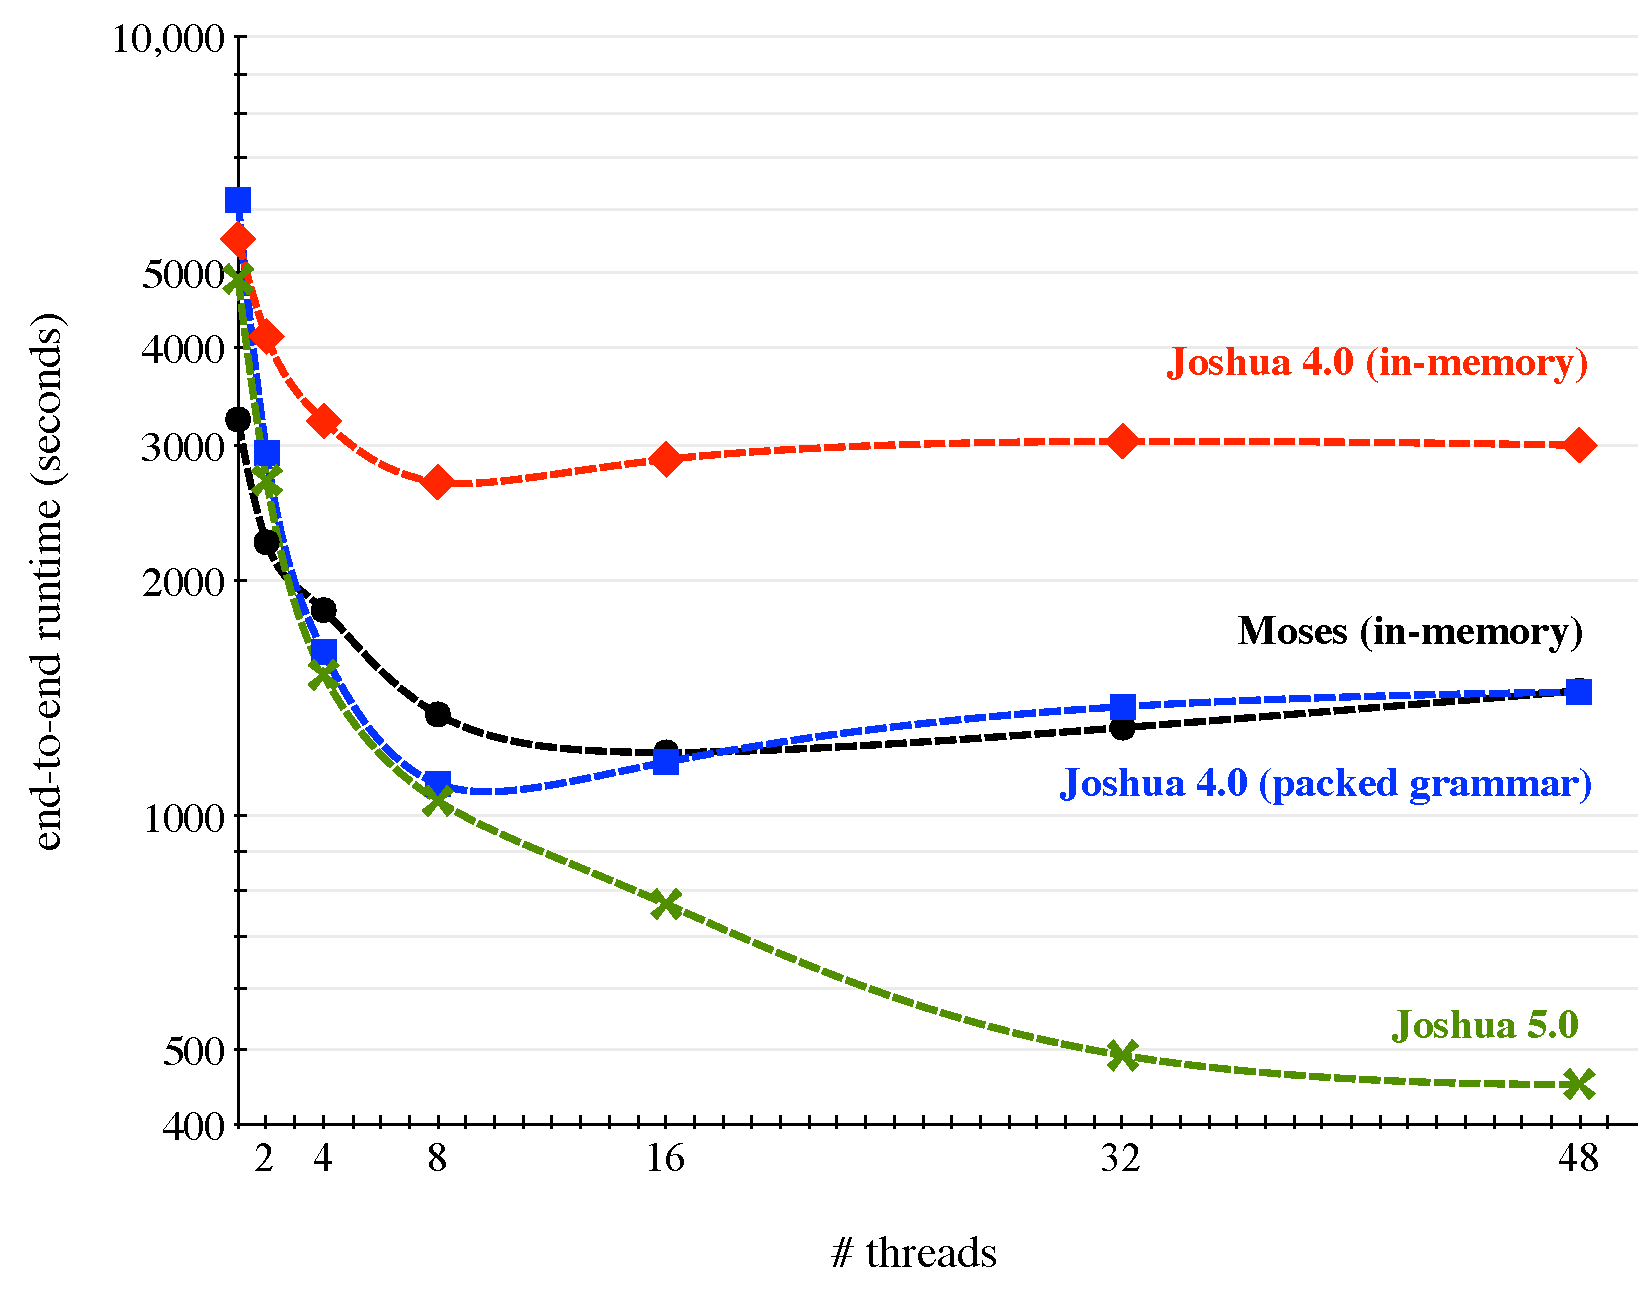
\includegraphics[width=0.99\linewidth]{figures/comparison.pdf}
  \end{center}
  \label{fig:cmp}
  \caption{End-to-end runtime as a function of the number of threads
    for Joshua 4.0 and Joshua 5.0.}
\end{figure}

\subsection{}



%%%%%%%%%%%%%%%%%%%%%%%%%%%%%%%%%%%%%%%%%%%%%%%%%%%%%%%%%%%%%%%%%
\section{Conclusion}

We present a new iteration of the Joshua machine translation
toolkit. Our system has been extended towards efficiently supporting
large-scale experiments in parsing-based machine translation and
text-to-text generation: Joshua 4.0 supports compactly represented
large grammars with its packed grammars, as well as large language
models via KenLM and BerkeleyLM.We include an implementation of PRO,
allowing for stable and fast tuning of large feature sets, and extend
our toolkit beyond pure translation applications by extending Thrax
with a large-scale paraphrase extraction module.

\paragraph{Acknowledgements}

This research was supported by in part by the EuroMatrixPlus project
funded by the European Commission (7th Framework Programme), and by
the NSF under grant IIS-0713448. Opinions, interpretations, and
conclusions are the authors' alone.

\bibliographystyle{acl2013}
\bibliography{joshua}

\end{document}
